\documentclass[a4paper,USenglish]{article}

\usepackage{microtype} %if unwanted, comment out or use option "draft"
 
% \usepackage{authblk}
 
% \pdfpagesattr{/CropBox [80 80 523 780]}
\pdfoutput=1
\usepackage[utf8]{inputenc}
%\usepackage{microtype}
\usepackage{amsmath}
\usepackage{amsthm}
\usepackage{amssymb}
\usepackage{float}
\usepackage[algoruled,linesnumbered,noend]{algorithm2e}
\usepackage{relsize}
\usepackage{enumitem}
\usepackage{cite}
\usepackage{multirow}
\usepackage{caption}
%\usepackage{subcaption}
\usepackage{url}
\usepackage{xspace}
\usepackage{graphicx}
\usepackage{booktabs}
\usepackage{mathcomp}
\usepackage{ifdraft}
\usepackage[external]{forest}
 
% REMOVE BEFORE SUBMISSION - begin part
% \usepackage{verbatim}
% \newcommand{\notaestesa}[2]{%
%   \marginpar{\color{red!75!black}\textbf{\texttimes}}%
%   {\color{red!75!black}%
%     [\,\textbullet\,\textsf{\textbf{#1:}} %
%     \textsf{\footnotesize#2}\,\textbullet\,]}%
% }
% \newcommand{\mynote}[2]{%
%   \marginpar{\color{red!75!black}\textbf{\texttimes}}%
%   {\color{red!75!black}%
%     [\,\textbullet\,\textsf{\textbf{#1:}} %
%     \textsf{\footnotesize#2}\,\textbullet\,]}%
% }
 
\usepackage{tikz}
\usetikzlibrary{shapes,arrows}
% \usetikzlibrary{snakes}
\usetikzlibrary{positioning,patterns}
\usepackage{ifpdf}
\usepackage{datetime}
\ifpdf%
\pdfinfo{%
  /Author (Author1;Author2)
  /Title (Title)
  /Keywords (perfect phylogeny;persistent perfect phylogeny)
  /CreationDate (D:\pdfdate)
}
\fi
 
\newcommand{\ie}{\emph{i.e.}}
 
\newtheorem{theorem}{Theorem}
\newtheorem{lemma}[theorem]{Lemma}
\newtheorem{proposition}[theorem]{Proposition}
\newtheorem{Observation}[theorem]{Observation}
\newtheorem{corollary}[theorem]{Corollary}
\newtheorem{Claim}[theorem]{Claim}
\newtheorem{property}[theorem]{Property}
\theoremstyle{definition}
\newtheorem{definition}{Definition}
\newtheorem{Problem}{Problem}
\newtheorem{Example}{Example}[section]

\title{\texttt{gpps}: An ILP-based approach for inferring cancer
  progression with mutation losses from single cell data}
\author{%
  Simone Ciccolella \and
  Mauricio Soto Gomez \and
  Murray Patterson \and
  Gianluca Della Vedova \and
  Iman Hajirasouliha \and
  Paola Bonizzoni}
\begin{document}
% \address{$^{1}$Department of Computer Science, Systems and Communication, Univ. Milano-Bicocca, Milan, Italy\\
% $^{2}$Institute for Computational Biomedicine, Department of Physiology and Biophysics, Weill Cornell Medicine of Cornell University, NY, USA\\
% $^{3}$Englander Institute for Precision Medicine, The Meyer Cancer Center, Weill Cornell Medicine, NY, US}

\maketitle

\begin{abstract}
  \noindent \textbf{Motivation:} In recent years, the well-known
  Infinite Sites Assumption (ISA) has been a fundamental feature of
  computational methods devised for reconstructing tumor phylogenies
  and inferring cancer progression where mutations are accumulated
  through histories.  However, some recent studies leveraging Single
  Cell Sequencing (SCS) techniques have shown evidence of mutation losses in several tumor samples~\cite{Kuipers13102017}, making the inference problem harder.\\
  \textbf{Results:} We present a new tool, \texttt{gpps}, that
  reconstructs a tumor phylogeny from single
  cell data, allowing each mutation to be lost at most a fixed number of times.\\
  \textbf{Availability:} The General Parsimony Phylogeny from Single
  cell (\texttt{gpps})
  tool is open source and available at   \url{https://github.com/AlgoLab/gppf}.\\
  % \textbf{Contact:} \href{s.ciccolella@campus.unimib.it}{s.ciccolella@campus.unimib.it}
  % \textbf{Supplementary information:} Supplementary data are available at \textit{Bioinformatics}online.}
\end{abstract}

\section{Introduction}

Recent developments of targeted therapies for cancer patients rely on
the accurate inference of the clonal evolution and progression of the
particular cancer. As discussed in several recent studies, such
as~\cite{Morrissy2016} and~\cite{Wang2016}, understanding the order of
accumulation and prevalence of somatic mutations during cancer
progression can help better devise therapeutic strategies.  Moreover,
studying the evolutionary history of tumors can provide some insights
on which mutations lead to drug resistance.

The most widely studied techniques for inferring cancer progression
rely on data from next-generation bulk sequencing experiments.  In
these cases, we sample mixtures of cells that are not homogeneous from
a mutational profile (\ie, which mutations appear in a cell) point of
view.  Moreover, we cannot easily distinguish between cells: the only
information we can have is, for each mutation, the fraction of cells
in a sample carrying such mutation.  Recently, many computational
approaches have been developed for the analysis of bulk-sequencing
data with the purpose of inferring tumoral subclonal decomposition and
reconstructing tumor phylogenies
(trees)~\cite{Strino2013,Jiao2014,Hajirasouliha2014,Yuan2015,Popic2015,citup,El-Kebir2016,marass2016,doi:10.1093/bioinformatics/btx270,Bonizzoni:2017:BPP:3107411.3107441},
but almost all of them model a tumor progression as the accumulation
of mutations under the Infinite Sites Assumption, that is recurrent
mutations and mutation losses are not allowed.

Single Cell Sequencing (SCS) greatly improves the resolution of the
data available, as it provides the set of mutations of each cell
analyzed.  However, this technique is currently expensive and not
especially reliable, since it produces datasets with a high amount of
noise that include allelic dropout (false negatives) and missing
values, due to lack of read coverage, as well as false positive calls
-- although this event is much rarer.  Another source of noise is due
to doublets, that is signals originating from two separate cells which
are erroneously inferred to originate from a single cell: we point out
this latter problem is fading away and can be tackled computationally.
Still, we need efficient methods that are able to cope with the kind
of data that SCS techniques are currently producing, by taming the
difficulties due to the noise in data.

Various methods have been developed for this
purpose~\cite{Jahn2016,Ross2016, Zafar2017}, some of them introducing
a hybrid approach of combining both SCS and VAF
data~\cite{Ramazzotti132183, Malikic234914, Salehi2017}.  As stated
before, most of these methods rely on the Infinite Sites Assumption
(ISA), which states that a mutation is acquired at most once in the
phylogeny and is never lost. The ISA was introduced
in~\cite{Kimura1969}.  This simplifying assumption also leads to a
computationally tractable model of evolution~\cite{gusfield1991}
called the perfect phylogeny.  Cancer progression, however, is a very
fast and aggressive form of evolution with limited data supporting
neutral evolution~\cite{DAVIS2017151}, with some studies showing
rather the evidence of selection~\cite{Bignell2010,DAVIS2017151} --
something that is particularly true in tumour samples after a
relapse~\cite{Ding2012,Gillies2012,DAVIS2017151}, where the tumour has
already been highly selected by the therapy targeted to destroy it.
Thus, one would be expect that we must abandon the strict Infinite
Sites Assumption in this setting, and indeed this is the case, as some
recent studies are finding hints suggesting that the ISA does not
always hold~\cite{Kuipers13102017,Brown2017,Bignell2010}.
In~\cite{Brown2017}, the authors find that large deletions on several
branches of a tree can span a shared locus, thus a given mutation may
be deleted independently multiple times.  In~\cite{Bignell2010}, the
authors show that in certain cases, homozygous deletions in cancer
genomes can even provide a selective growth advantage. Each
(independent) deletion of an acquired mutation takes us further away
from the ISA. Some recent methods such as
TRaIT~\cite{Ramazzotti132183} and SiFit~\cite{Zafar2017} allow
deletions of mutations.

The Dollo model~\cite{Rogozin2006} of evolution is designed exactly
for some of the cases where a perfect phylogeny does not represent the
actual data.  More precisely, the Dollo model requires each mutation
to be acquired exactly once in the entire history analyzed, while
removing all restrictions on the number of times that a mutation can
be lost.  The Dollo model as well as the Dollo($k$) variants, where
each mutation can be lost at most $k$ times, has been introduced
recently in the literature on algorithmic approaches for tumor
progression
inference~\cite{Bonizzoni:2017:BPP:3107411.3107441,Ciccolella268243}.
Unfortunately, the Dollo model does not have the convenient
computational tractability of the perfect phylogeny
model~\cite{gusfield1991}, hence requiring more sophisticated
algorithms.

In this paper we propose (\texttt{gpps}), a tool of the \texttt{gppf}
family, that exploits an Integer Linear Programming (ILP) approach to
infer a tumor progression that can include mutation losses, from
single cell sequencing data.

\section{Tumor phylogeny reconstruction from single cell data}

In the most abstract formulation, we can see the cancer progression
reconstruction problem as a character-based phylogeny reconstruction
problem~\cite{Gusfield} where each character represents the
presence/absence of a specific mutation in a cell.

\begin{figure}[tb!]
  \begin{minipage}[c]{0.55\textwidth}
    \includegraphics{img/dollo_example-figure0}
  \end{minipage}
  \begin{minipage}[t]{0.3\textwidth}
    \begin{tabular}[!t]{c|ccccccc}
      & a & b & c & d & e & f & g  \\ \hline
      $s_1$ & 1 & 1 & 1 & 0 & 0 & 0 & 0 \\
      $s_2$ & 1 & 0 & 0 & 0 & 1 & 0 & 0 \\
      $s_3$ & 0 & 1 & 0 & 1 & 0 & 1 & 0 \\
      $s_4$ & 1 & 0 & 0 & 0 & 0 & 0 & 1
    \end{tabular}
  \end{minipage}
  \caption{Example of a binary matrix that does not allow a perfect
    phylogeny, since columns $a$ and $b$ are in conflict, \ie, the
    four gametes rule~\cite{gusfield1991} does not hold. The tree
    represents one of the possible Dollo phylogenies that explain the
    matrix.}
  \label{fig:dollo}
\end{figure}

The input of the problem is an incomplete binary matrix $I$, where the
entry $I[c,m]=0$ indicates that the cell $c$ does not have the
mutation $m$, while $I[c,m]=1$ indicates that the cell $c$ has the
mutation $m$.  Finally, we denote with $I[c,m]=\ ?$ where there is not
enough information on the presence/absence of mutation $m$ in cell
$c$.  We recall that uncertainty about the presence of a mutation in a
cell is a consequence of insufficient coverage in the sequencing,
hence it is unavoidable.

However, uncertainty is not the only issue in the sequencing process:
the input matrix $I$ also contains false positives and false
negatives.  We assume that these errors occur independently and
uniformly across all the (known) entries of $I$.  Namely, $P$ denotes
the predicted matrix, \ie, the binary matrix without missing values
computed by the algorithm.  In this case, $\alpha$ denotes the false
negative rate and $\beta$ denotes the false positive rate.  In other
words, for each pair $(c,m)$,
\begin{itemize}
\item $Pr(I[c,m] = 0|P[c,m] = 0) = 1- \beta$
\item $Pr(I[c,m] = 1|P[c,m] = 0) = \beta$
\item $Pr(I[c,m] = 1|P[c,m] = 1) = 1- \alpha$
\item $Pr(I[c,m] = 0|P[c,m] = 1) = \alpha$
\end{itemize}

Our goal is to find a matrix $P$ that (1) corresponds to a phylogeny
on the set of cells, and (2) maximizes the the likelihood

\begin{equation}
  \label{eq:likelihood}
  Pr(I|P) = \prod_{c} \prod_{m} Pr(I[c,m] | P[c,m])
\end{equation}

of the observed matrix $I$~\cite{Jahn2016}.  In other words, we want
to find the phylogeny, as expressed by the matrix $P$, that maximizes
the likelihood of the observed matrix $I$~\cite{Jahn2016}.  We point
out that the values of the unknown entries of the input matrix do not
factor into the objective function.
% Thus, $Pr(I[c,m] = ?|P[c,m] = 1) = Pr(I[c,m] = ?|P[c,m] = 0) = 1$.

A phylogeny is a rooted labeled tree $T$, where the label set
corresponds to the set of mutation gains and losses.  The state $S(x)$
of a leaf $x$ in $T$ is defined as the set of mutations that are
acquired and not lost in the path from the root of $T$ to $x$.  We say
that the tree $T$ encodes a matrix $P$ if there exists a mapping
$\sigma$ of the rows of $P$ to the leaves of $T$ such that for each
row $r$ of $P$, it follows that $C(r)=S(\sigma(r))$ where $C(r)$ is
the set of columns which are 1 in $r$, and $\sigma(r)$ denotes the
leaf of $T$ associated with $r$ through $\sigma$.  In other words, in
the tree $T$ we assume that the cell $c$ has been extracted from the
subpopulation $\sigma(c)$.  See Figure~\ref{fig:dollo} for example of
a phylogeny a matrix that it encodes.

\begin{figure}[!tb]
  \begin{minipage}{0.72\linewidth}
    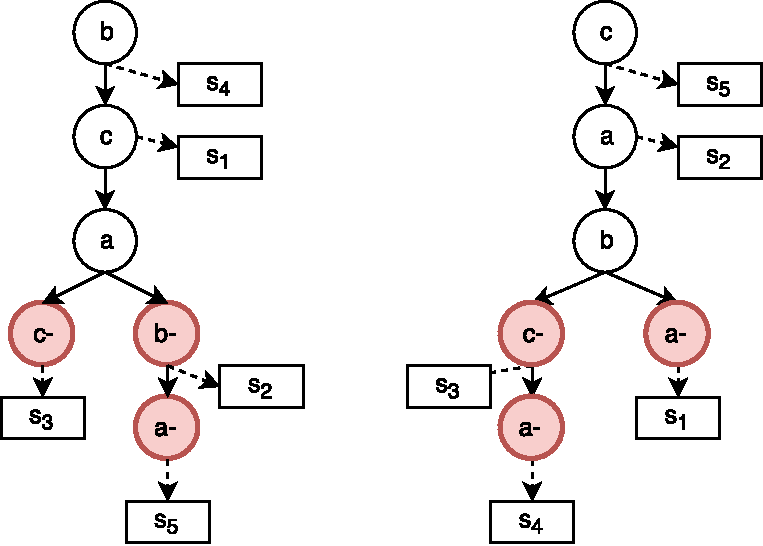
\includegraphics[scale=.65]{img/dollo_non_unique}
  \end{minipage}
  \begin{minipage}{0.2\linewidth}
    \begin{tabular}[!t]{c|ccc}
      & a & b & c \\ \hline
      $s_1$ & 0 & 1 & 1 \\
      $s_2$ & 1 & 0 & 1 \\
      $s_3$ & 1 & 1 & 0 \\
      $s_4$ & 0 & 1 & 0 \\
      $s_5$ & 0 & 0 & 1
    \end{tabular}
  \end{minipage}
  \caption{Example of two Dollo phylogenies that explain the same
    binary matrix.  It is important to notice that the ancestral order
    of mutations $c,a$ and $b$ is inverted but the two different trees
    can equally explain the input binary matrix. In fact, in a Dollo
    phylogeny the order of two mutations can be inverted and, thank to
    the introduction of deletions, they could both be correct
    solutions for a given input.  }
  \label{fig:dollo_non_unique}
\end{figure}

We can express the likelihood of the matrix $P$ as in
Equation~\ref{eq:likelihood} --- since the involved probabilities are
in [0,1] it is convenient to move to a (linear) log-likelihood
maximization objective function of the form:

\begin{equation}
  \label{eq:log-likelihood}
  \mbox{max } \sum_c \sum_m \log Pr\left( I[c,m] | P[c,m]\right)
\end{equation}

\subsection{The evolution model}
\label{sec:intro_dollok}

The Dollo parsimony rule can be interpreted as the impossibility of
having an identical mutation in the evolutionary trajectory.  This
rule can be translated in the phylogeny tree model as the unique
introduction of any single mutation but any number of deletions of
this mutation.

From an algorithmic point of view, phylogeny reconstruction with a
Dollo evolutionary model is an NP-complete
problem~\cite{BKW95,DAY198633}.  A hierarchical chain of restricted
versions of the model can be obtained by bounding the number of
deletions for each character.  We denote as Dollo($k$) the
evolutionary model in which each mutation can be acquired exactly once
and can be lost at most $k$ times.  In this way Dollo($0$) and
Dollo($1$) correspond to the perfect and persistent phylogeny models,
respectively.  In the tree generation process for the Dollo($k$) model
($k>0$) we are required to augment a Perfect phylogeny representing
the cancer progression by adding nodes which represent the loss of a
mutation, \ie, a node labelled $m^-_l$, representing the $l$-th loss
of mutation $m$.  The state of the leaf $x$ is the set of mutations
$m$ that, in the path from the root to $x$, have been acquired --- the
path has a vertex labeled $m^{+}$ --- but never lost --- the path has
no vertex labeled $m_{i}^{-}$.  We stress that, when deletions are
introduced, the set of feasible phylogenies which represent a given
solution is no longer unique as in the case of Perfect phylogeny ---
See Figure~\ref{fig:dollo_non_unique} for an example.
% We can see that switching the labels of nodes $b^-$ and $d^-$ in Figure~\ref{fig:dollo} produces a different tree which is still a solution of the proposed input matrix. 
% Moreover we see that ancestral relationship between characters is different in both representations.
% When the number of cells, mutations and possible deletions increases, and with the noise caused by false calls and missing entries, this problem is greatly amplified, causing the number of different cancer progression phylogenies which equally explain the same input, to explode. A more complex example can be seen in Figure~\ref{fig:dollo_non_unique} where a different order of mutations and a different set of deletions can equally explain a given input.

Testing if an incomplete matrix $I$ has a phylogeny under the
Dollo($k$) model has been attacked via ILP for
$k=0$~\cite{Gusfield2007}, $k=1$~\cite{gusfield_persistent_2015}, and
for general $k$~\cite{Bonizzoni:2017:BPP:3107411.3107441}.  We will
exploit the latter formulation to describe an ILP approach for tumor
phylogeny reconstruction from single cell data.

% The character-based phylogeny reconstruction problems we study in this
%   paper are constrained versions of the general Incomplete Directed
%   Perfect  Phylogeny (IDP)~\cite{Peer_2004}.
% The IDP problem asks for completing missing data in a binary matrix, where
%   missing data are represented by the symbol $?$, in such a way that the
%   completed matrix is explained by a perfect phylogeny.
% More precisely, the input data is an $n\times m$ matrix $M_{?}$, where
%   $M_{?}(i,j)\in \{0,1,?\}$ represents the absence, presence or
%   uncertainty of a character $j$ in the species $i$ respectively.
% If a solution  exists, then it consists of changing  each $?$ into $0$
%   or $1$  obtaining a new  binary matrix  $M_{s}$ that has  a directed
%   perfect phylogeny. 

First, we recall that a well known characterization of perfect
phylogenies states that a \emph{complete} binary matrix $M$ has a
directed perfect phylogeny if and only if it has no \emph{conflicting}
pair of columns --- two columns are in conflict if they contain all
three configurations $(0,1)$, $(1,0), (1,1)$ --- inducing the
so-called forbidden matrix (\emph{c.f.} Figure~\ref{fig:dollo}).

The ILP formulation on \emph{incomplete} matrices~\cite{Gusfield2007}
essentially consists of introducing a binary variable for each missing
entry, and describing a set of constraints towards the goal of
minimizing the conflicting pairs.

To adapt this approach to persistent
phylogenies~\cite{gusfield_persistent_2015}, we need a
property: 

\begin{proposition}
  \label{proposition:extended matrix}
  \cite{Bonizzoni:2017:BPP:3107411.3107441} Let $M$ be an incomplete
  binary matrix.  Let $M_{e}$ be the (incomplete) matrix obtained from
  $M$ as follows: for each entry $M[i,j]$ we have $k+1$ entries
  $M_{e}[i,j^{+}]$ and $M_{e}[i,j_{l}^{-}]$ (for $1\le l\le k$) such
  that (1) if $M[i,j] = 1$ then $M_{e}[i,j^{+}] = 1$ and
  $M_{e}[i,j_{l}^{-}] = 0$ for $1\le l\le k$, (2) if $M[i,j] = 0$ then
  the entries $M_{e}[i,j^{+}]$, $ M_{e}[i,j_{l}^{-}]$ are all missing.
  Then $M$ has a completion $M^{*}$ that has a Dollo$(k)$ phylogeny if
  and only if $M_{e}$ has a completion $M^{*}_{e}$ such that if
  $M(i,j)= 0$ then
  $M^{*}_{e}[i,j^{+}] = \sum_{l\le k} M^{*}_{e}[i,j_{l}^{-}]$.  See
  Figure~\ref{fig:M_e} for an illustration.
\end{proposition}

Our main contribution is combining the ILP formulation
of~\cite{Bonizzoni:2017:BPP:3107411.3107441} with the definition of
tumor perfect phylogeny reconstruction from single cell data, to
obtain an ILP approach for tumor phylogeny reconstruction from single
cell data that incorporates mutation losses in the model.

% This relation motivates the following definition~\cite{gusfield_persistent_2015}:

%   \begin{definition}\label{def:MIDPP}
%     Let $M_{e}$ be an incomplete binary matrix, and let 
%     $\mathcal{R}=\{R_i(M_e)\le 0\}_{i\in [1,r]} $  be a set 
%     of $r$ constraints on the entries of $M_e$.
% %
% Then the \emph{Modified Incomplete Directed Perfect Phylogeny Problem for the set}
%     $\mathcal R$, denoted by MIDPP($M_e,\mathcal R$),  asks to find, if it exists,
%      a completion of matrix $M_e$ which admits a Perfect Phylogeny and 
%    satisfies all constraints in $\mathcal R$.
% %
%   \end{definition}


% \section{The $\boldsymbol{\mathcal P}$ Incomplete Directed Phylogeny 
%     Problem }
%   \label{sec:ILP_general}

% In  this section  we  develop  an ILP  formulation  for  the following  
% problem:

% \begin{definition}[${\mathcal P}$ Incomplete Directed Phylogeny 
%     Problem]
%   \label{definition:p-idpp}
% Given a character-based phylogeny model $\mathcal P$ and an incomplete binary matrix
% $M$, the ${\mathcal P}$ Incomplete Directed Phylogeny 
% Problem, denoted by $\mathcal P$-IDP, asks for a
% completion $M_{c}$ of $M$, such that $M_{c}$ admits a phylogeny $T$ under 
%     the model $\mathcal P$, if such a completion exists.
% %
% \end{definition}
 
% Notice that if all entries of the input matrix $M$ are
% known,  then the  problem corresponds  to deciding  if $M$  admits a phylogeny
% under the model $\mathcal P$.  
% In this paper we focus on Dollo($k$) and Camin-Sokal($k$).
% As  we have  already  mentioned, we  proceed by  reducing  the $\mathcal  P$-IDP
% on an instance $M$ to an equivalent MIDPP($M_e$,$\mathcal R_M$) instance where 
% $M_e$  is a  related extended  matrix  and $\mathcal  R_M$  is a  set of  linear
% restrictions. The later problem can thus be restated as an ILP. 
  
% \subsection{The Dollo($\boldsymbol{k}$)-IDP} 
% \label{sec:ilp_Dollo}

%   \subsubsection{Extended        Matrix        and        Constraints        for
%     Dollo$(k)$}\label{sec:dollok_M}

% The results in this section are from~\cite{Bonizzoni:2017:BPP:3107411.3107441}.

  
% Let  $M$ be a binary (incomplete) matrix with $n$ rows (species) and $m$ characters.  
% The extended matrix $M_{D(k)}$ for the Dollo($k$) model is defined as
% follows:  
% \begin{itemize}
%   \item $M_{D(k)}$ has $n$ rows and  $m\times(k+1)$ columns, where each
%     character $j$ of matrix $M$ is associated to $k+1$ columns in  $M_{D(k)}$
%     denoted by  $j^{+},j^{-}_1,\ldots,j^{-}_{k}$. 
%   \item If $M(i,j)=1$
%     then $M_{D(k)}(i,j^{+})=1$ and $M_{D(k)}(i,j^{-}_l)=0,\, l\in [1,k]$.
%   \item If  $M(i,j)=0$ or  $M(i,j)=?$ then $M_{D(k)}(i,j^{+})=?$ and
%     $M_{D(k)}(i,j^{-}_l)=?$  for each  $l \in [0,k]$. 
%   \end{itemize}

% For a character $j$, the column $j^{+}$ represents the acquisition of
%   character $j$ while each of the  $j^{-}_{1} \cdots j^{-}_{k}$ columns represents a
%   possible loss of the gained character.
% If  $M(i,j)=1$, then it is  not possible for species $i$ to lose the
% character $j$, thus the  only possible  configuration is  $M_{D(k)}(i,j^{+})=1$ and
% $M_{D(k)}(i,j^{-}_l)=0,\, l\in [1,k]$. 
% Otherwise, if $M(i,j)=0$ then the character has either (1) never been acquired, or (2) been
% acquired, then lost along the path from the root to the species $i$ of any solution.
% %
% Therefore $ \sum_{1\le l\le
%   k}M_{D(k)}(i,j^{-}_l)=M_{D(k)}(i,j^{+})$. 

% Finally, if $M(i,j)=?$, that is the entry of $M$ is missing,  we must allow both the
% constraints for the case $M(i,j)=0$ as well as $M(i,j)=1$.
% %
% % consider both of the aforementioned relations,
% % that is $(M_{D(k)}(i,j^{+})=1 \wedge \sum_{1\le l\le
% %   k}M_{D(k)}(i,j^{-}_l)=0) \vee (\sum_{1\le l\le
% %   k}M_{D(k)}(i,j^{-}_l)=M_{D(k)}(i,j^{+}))$. 
% We capture both cases with with following relation
% between the entries of the extended matrix:
% $ 0\le M_{D(k)}(i,j^{+}) - \sum_{1\le l\le k}M_{D(k)}(i,j^{-}_l)\le 1$.
% Our previous discussion  leads to the  following set  of constraints for  the matrix
% $M_{D(k)}$:
% %\begin{equation}\label{eq:R_Dk}
% % \medmuskip=0mu
% % \thinmuskip=0mu
% % \thickmuskip=0mu
% %\scalebox{.9}{
% {\small \begin{align} \label{eq:R_Dk}
% &\mathcal{R}_{D(k)}(M)=\left\{\sum\limits_{1\le l\le k}M_{D(k)}(i,j^{-}_l)=
%   M_{D(k)}(i,j^{+})\right\}_{(i,j): M(i,j)=0} \nonumber\\
% &\quad \cup \left\{0 \le\sum\limits_{1\le l\le k}M_{D(k)}(i,j^{-}_l)-
%   M_{D(k)}(i,j^{+})\le 1\right\}_{(i,j): M(i,j)=?}
% \end{align}
% }  
% %\end{equation}

% By an abuse of the notation it is possible to describe all restriction for the problem as:
% \begin{equation}\label{eq:Dk2}
%   M_{D(k)}(i,j^{+}) - \sum_{1\le l\le k}M_{D(k)}(i,j^{-}_l)= M(i,j),
% \end{equation}
% where the case $M(i,j)=?$ is interpreted as $M_{D(k)}(i,j^{+}) - \sum_{1\le l\le k}M_{D(k)}(i,j^{-}_l)\in \{0,1\} $.

% When  the  context  is  clear,  we  will denote  this  set  of  restrictions  as
% $\mathcal{R}_{D(k)}$. 
% Figure~\ref{fig:M_e} shows an example of the input matrix and its
% corresponding extended matrix.

% \begin{theorem}\label{theorem:dollok}
%   Let $M$ be an incomplete binary matrix, and let MIDPP$\left(M_{D(k)},\mathcal
%     R_{D(k)}(M)\right)$ be the corresponding incomplete instance in the 
%   extended matrix $M_{D(k)}$.
% %
% Then there exist a completion $M_{c}$ of $M$ satisfying the Dollo($k$) model if
% and only if MIDPP$\left(M_{D(k)},\mathcal R_{D(k)}(M)\right)$ admits a solution.

% Moreover, from  any Dollo($k$) completions  $M_{c}$ it is possible to  obtain a
% solution of MIDPP$\left(M_{D(k)},\mathcal R_{D(k)}(M)\right)$ and vice versa.
% \end{theorem}

\begin{figure}[tb!]
  \begin{minipage}[b][30pt][c]{0.3\linewidth}
    \flushright
    \scalebox{.92}{
      \begin{tabular}{c|ccc}
        & $a$ & $b$ & $c$  \\
        \hline
        1& ? & 0 & 0 \\
        2& 0 & 1 & 0 \\
        3& 0 & 0 & 1 \\
        4& 1 & 1 & ? \\
        5& 0 & ? & 1 \\
        6& 1 & 0 & 1 \\
      \end{tabular}
    }\\[20pt]
    
    \scalebox{.92}{
      \begin{tabular}{c|ccc}
        & $a$ & $b$ & $c$  \\
        \hline
        1& 1 & 0 & 0 \\
        2& 0 & 1 & 0 \\
        3& 0 & 0 & 1 \\
        4& 1 & 1 & 0 \\
        5& 0 & 1 & 1 \\
        6& 1 & 0 & 1 \\
      \end{tabular}  
    }
  \end{minipage}
  \begin{minipage}[c]{.65\linewidth}
    \centering
    \includegraphics[width=\textwidth]{img/Dollo2tree}\\\vspace{1em}    
  \end{minipage}
  
  \begin{minipage}{.5\linewidth}
    \scalebox{.92}{
      \begin{tabular}{p{1pt}|p{1pt}p{1pt}p{1pt}p{1pt}p{1pt}p{1pt}p{1pt}p{1pt}p{1pt}}%{c|ccccccccc}
        &$a_0$&$a_1$&$a_2$&$b_0$&$b_1$&$b_2$&$c_0$&$c_1$&$c_2$\\\hline
        1& ? & ? & ? & ? & ? & ? & ? & ? & ? \\
        2& ? & ? & ? & 1 & 0 & 0 & ? & ? & ? \\
        3& ? & ? & ? & ? & ? & ? & 1 & 0 & 0 \\
        4& 1 & 0 & 0 & 1 & 0 & 0 & ? & ? & ? \\
        5& ? & ? & ? & ? & ? & ? & 1 & 0 & 0 \\
        6& 1 & 0 & 0 & ? & ? & ? & 1 & 0 & 0 
      \end{tabular} 
    }
  \end{minipage}
  \begin{minipage}{.5\linewidth}
    \scalebox{.92}{
      \begin{tabular}{p{1pt}|p{1pt}p{1pt}p{1pt}p{1pt}p{1pt}p{1pt}p{1pt}p{1pt}p{1pt}}
        & $a_0$ &$a_1$ &$a_2$ & $b_0$ &$b_1$ &$b_2$ &$c_0$ &$c_1$ &$c_2$ \\
        \hline
        1& 1 & 0 & 0 & 0 & 0 & 0 & 0 & 0 & 0 \\
        2& 1 & 1 & 0 & 1 & 0 & 0 & 1 & 1 & 0 \\
        3& 1 & 0 & 1 & 1 & 1 & 0 & 1 & 0 & 0 \\
        4& 1 & 0 & 0 & 1 & 0 & 0 & 0 & 0 & 0 \\
        5& 1 & 1 & 0 & 1 & 0 & 0 & 1 & 0 & 0 \\
        6& 1 & 0 & 0 & 1 & 1 & 0 & 1 & 0 & 0 \\
      \end{tabular}
    }
  \end{minipage}

  \caption{An input matrix $M$ (top left), a Dollo(2) completion $M_c$ (center
  left) and its corresponding phylogeny tree $T$ (top right). 
  The $M_{D(2)}$ extended matrix (bottom left) 
  and a completion for the MIDPP($M_{D(2)},\mathcal R_{D(2)})$
  according to Proposition~\ref{proposition:extended matrix}.
%
  In the tree, boldfaced character corresponds to changes between each
  node and its parent.  }
\label{fig:M_e}
\end{figure}

\section{The ILP formulation}
\label{sec:ilp}
In this section we present our ILP formulation for the tumor phylogeny
reconstruction from single cell data.

We recall that the input of the problem is an incomplete matrix $I$
represented as a set of binary variables $I(c,m)$ such that $I(c,m)=1$
if cell $c$ has (according to the input data) the mutation $m$, while
$I(c,m)=0$ if cell $c$ does not have (according to the input data) the
mutation $m$.
%
Notice that the input data is incomplete, hence we can have pairs
$(c,m)$ such that the variable $I(c,m)$ does not exist.

The variables $P(c,m^{+})$ and $P(c,m_{i}^{-})$ encode the extended
matrix that we want to compute and that will satisfy
Proposition~\ref{proposition:extended matrix}.  Differently from the
variable $I(\cdot,\cdot)$, for each pair $(c,m)$, all variables
$P(c,m^{+})$ and $P(c,m_{i}^{-})$ exist.

We introduce some auxiliary variables that help in making the ILP
formulation easier to read.  The binary variables $F(c,m)$ indicates
if, in the predicted matrix, the cell $c$ has the mutation $m$.  By
Proposition~\ref{proposition:extended matrix}, $F(c,m)=1$ if and only
if $P(c,m^{+})=1$ and all $P(c,m_{i}^{-})$ are equal to zero.
Moreover, the real variables $w(c,m)$ represent the probability of
$P(c,m)$ given $I(c,m)$ --- the formula of the actual values depends
on the possible cases, that is if we have a true positive, a true
negative, a false positive, and a false negative.

To establish if two columns are in conflict, we introduce the final
binary variables $B(p,q,a,b)$, which are defined for each pair of
columns $(p,q)$ and for each possible pair of values
$(a,b)\in \{(0,1), (1,0), (1,1)\}$.  More precisely, $B(p,q,a,b)$
indicates if for the pair $(p,q)$ of columns there exists a cell $c$
where $P(c,p)=a$ and $P(c,q)=b$.  Notice that two columns $p$ and $q$
are conflicting iff $B(p,q,0,1) + B(p,q,1,0) + B(p,q,1,1) = 3$.  We
are now ready to introduce our ILP formulation, where we use $C$ to
denote the set of cells (\ie, the rows of the input matrix $I$), $M$
to denote the mutations (\ie, the columns of $I$), and $M^{*}$ to
denote the set of possible mutation gains or losses.

\begin{align}
  \max \sum_{c\in C}\sum_{m\in M}\log w(c,m),\text{ subject to }&\notag\\
  F(c,m) = P(c,m^{+}) - \sum_{i\le k} P(c, m_{i}^{-}) &\ \forall c\in C,\ m\in M\label{eq:def-F}\\
  w(c,m) = \left(1 - \alpha\right) F(c,m) +  \beta \left( 1 - F(c,m) \right)\quad&\text{ if } I(c,m) = 1\label{eq:cost-FP}\\
  w(c,m) = \alpha F(c,m) +  \left(1 - \beta\right) \left( 1 - F(c,m) \right)\quad&\text{ if } I(c,m) = 0\label{eq:cost-FN}\\
  B(p,q,0,1)\ge P(c,q) - P(c,p) \quad&\ \forall c\in C,\ p,q\in M^{*}\label{eq:case-01}\\
  B(p,q,1,0)\ge P(c,p) - P(c,q) \quad&\ \forall c\in C,\ p,q\in M^{*}\label{eq:case-10}\\
  B(p,q,1,1)\ge P(c,p) + P(c,q) -1 \quad&\ \forall  c\in C,\ p,q\in M^{*}\label{eq:case-11}\\
  B(p,q,0,1) + B(p,q,1,0) + B(p,q,1,1)\le 2  \quad&\forall  p,q\in M^{*}\label{eq:no-conflict}\\
  B(\cdot,\cdot,\cdot,\cdot), F(\cdot,\cdot), P(\cdot,\cdot)&\in \{0,1\}\notag
\end{align}

% The goal is to decide if there exists a completion of the unknown
% entries  of $I$ resulting in
% a (complete) matrix  admitting a Perfect Phylogeny.
% The main  strategy of  this approach  is to state  the problem  as the
%   minimization of the conflicts between pairs of characters. 
% Thus, in virtue of the  Perfect Phylogeny Theorem, the IDP problem
% will have a solution if and only if the cost of the minimization problem
% is zero.  

% % In what follows, we  briefly explain the key elements of the  ILP and we discuss
% % the required changes for its use in the MIDPP problem.

% Since the objective is to determine if two columns are in conflict,
%   for every pair of columns $p,q$ we define a  binary variable $C(p,q)$
%   which indicates the existence of a conflict between these two columns.
% To establish if two columns are in conflict, we introduce the binary variables 
%    $B(p,q,a,b)$, which  are defined for each pair of columns $(p,q)$ and for each
%    possible  pair  of  values  $(a,b)\in \{0,1\}^2$.
% The variable $B(p,q,a,b)$ indicates if for the (ordered) pair of columns $(p,q)$
%   there  exists a cell $c$ where $P(c,p)=a$ and $P(c,q)=b$.
% Moreover, if there exist two cells $c_{1}$ and $c_{2}$ such that 
%   $P(c_{1},p)=a$ and $P(c_{2},q)=b$, then $B(p,q,a,b)=1$.

% For each pair $(p,q)$ of columns, for each pair $(a,b)\in
% \{(1,0),(0,1),(1,1)\} $, and for each cell $c$, the following set of inequalities 
% \begin{equation}\label{eq:B}
%    B(p,q,a,b)\ge 1-[a+(-1)^{a} P(c,p)]-[b+(-1)^{b}
%   P(c,q)]
%   \end{equation}
%   forces the variable $B(p,q,a,b)$ to be $1$ if and only if the columns $p,q$
%   exhibit the pair $(a,b)$ in some row $i$.

% Since we want phylogenies that correspond to extended matrices without conflicts,
% we  will  consider  the   following  alternative  form  of  the  previous
% constraint: 
% \begin{equation}\label{eq:C=0}
%    B(p,q,0,1) + B(p,q,1,0) + B(p,q,1,1)\le 2.  
% \end{equation}

% We denote with $w(c,m)$ the contribution of the cell $c$ and the mutation $m$ to the
% objective function.
% If $M(c,m)=1$, then $w(c,m) = \left(1 - \alpha\right) \left( P(c,m^{+}) - \sum_{i} P(c, m_{i}^{-}) \right)
% +  \beta \left( 1 - P(c,m^{+}) - \sum_{i} P(c, m_{i}^{-}) \right)$.
% Symmetrically, if  $M(c,m)=0$, then $w(c,m) = \alpha \left( P(c,m^{+}) - \sum_{i} P(c, m_{i}^{-}) \right)
% +  \left(1 - \beta\right) \left( 1 - P(c,m^{+}) - \sum_{i} P(c, m_{i}^{-}) \right)$.


% The objective function that we want to maximize becomes:
% \begin{equation}
% \label{eq:log-likelihood-goal}
%     \mbox{max } \sum_c \sum_m \log w(c,m).
% \end{equation}

The total number of variables and constraints in the formulation are
$O(nm+m^2)$ and $O(nm^2)$ respectively.

\subsection{ILP implementation: gpps}

Our approach has been implemented with a Python program called
\texttt{gpps}.  The code, data and scripts used in our experimental
analysis is available at \url{https://github.com/AlgoLab/gppf}.  The
algorithm receives as input a frequency matrix $F$, the evolution
model (Persistent, Dollo($k$), Camin-Sokal($k$)) to be considered and
the maximum number of clones in the clonal matrix (expressed as the
percentage of the total number of mutations).  The program generates
the ILP formulation which is fed to an ILP solver in order to get the
optimal solution.

In our experiments we have used Gurobi~6.5.2 as the ILP solver.
Moreover, from the computed solution the program can construct the
corresponding solution tree, provided that feasible solution has been
found.
% We include the option of exporting the formulation as a standard LP file to be
%   processed by other another ILP solver.
Additionally, we have introduced a timeout on the running time, since
the generated ILP problem could be large and its resolution could
require a considerable amount of time.
%
We exploit the fact that Gurobi can be halted at any time and it
returns the best feasible solution computed so far.
%
Hence, imposing a timeout allows the ILP solver to compute a solution
with a small total error.

\section*{Acknowledgement}

SC acknowledges a Mobility Exchange Fellowship from the University of
Milano-Bicocca. Part of this work has been done during SC visit at
Weill Cornell.  This work was also supported by start up funds (Weill
Cornell Medicine) to IH.

% \bibliography{references}{}
% \bibliographystyle{natbib}
%\bibliographystyle{achemnat}
%\bibliographystyle{plainnat}
%\bibliographystyle{abbrv}
% \bibliographystyle{bioinformatics}
%
\bibliographystyle{plain}
\bibliography{references,singlecell}
\end{document}
